\documentclass[tikz,border=10pt]{standalone}

\usepackage{tikz}
\usetikzlibrary{positioning,fit,calc,shapes.geometric}

\begin{document}

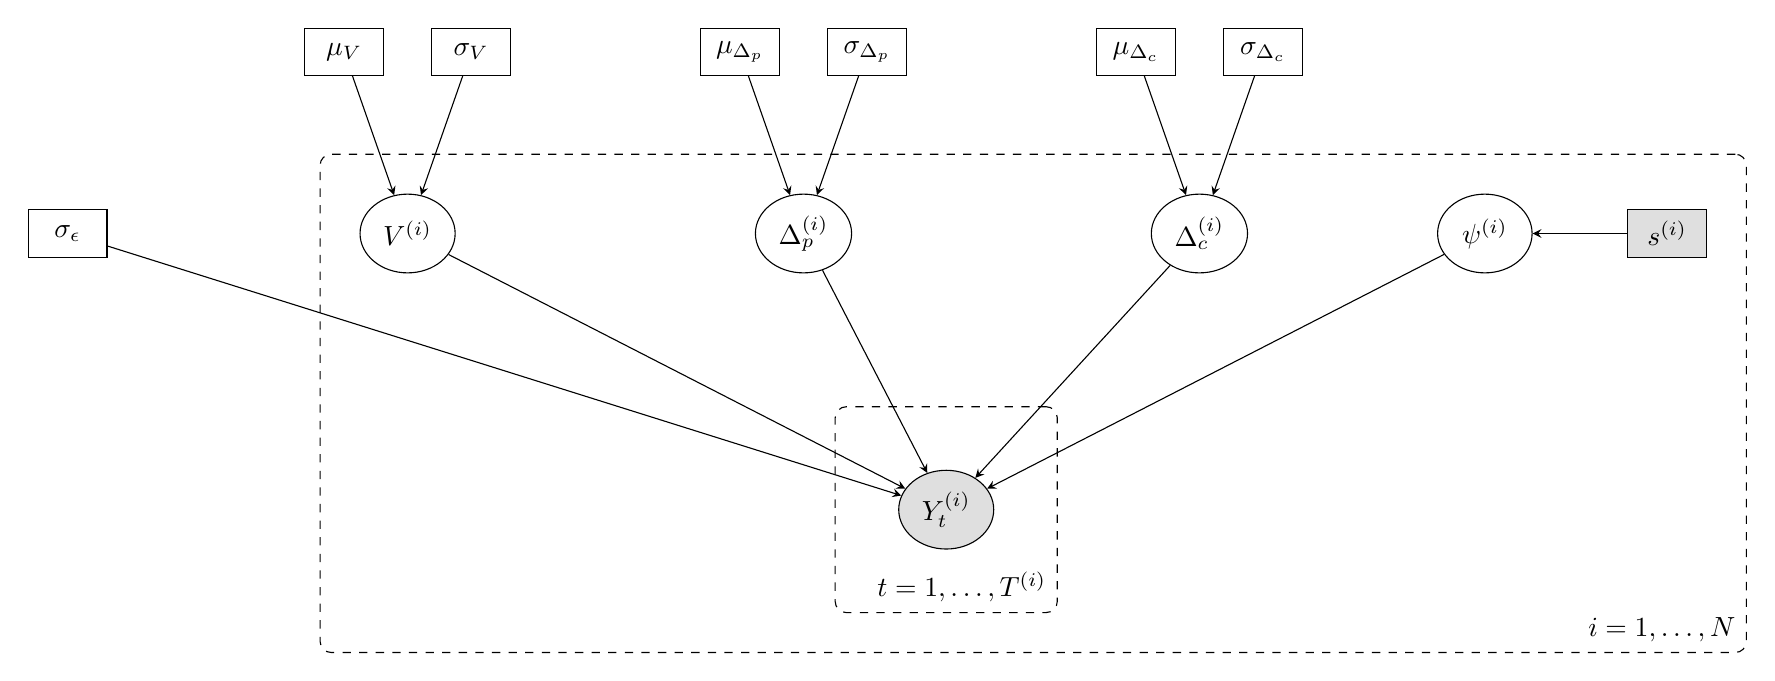
\begin{tikzpicture}[
    >=stealth,
    latent/.style={
        draw,
        shape=ellipse,
        minimum width=1.2cm,
        minimum height=1cm
    },
    obs/.style={
        draw,
        shape=ellipse,
        fill=gray!25,
        minimum width=1.2cm,
        minimum height=1cm
    },
    hyper/.style={
        draw,
        rectangle,
        minimum width=1.0cm,
        minimum height=0.6cm
    },
    known/.style={
        draw,
        rectangle,
        fill=gray!25,
        minimum width=1.0cm,
        minimum height=0.6cm
    },
    plate/.style={
        draw,
        dashed,
        rounded corners,
        inner sep=0.5cm
    }
]

%%%%%%%%%%%%%%%%%%%%%%%%%%%%%%%%%%%%%%%%%%%%%%%%%%%%
%% Population level
%%
%% Each (mu, sigma) pair governs a lognormal over the individual values:
%% mu is the median and sigma the natural-scale spread, converted to the
%% log-scale multiplier sigma/mu inside the model.
%%%%%%%%%%%%%%%%%%%%%%%%%%%%%%%%%%%%%%%%%%%%%%%%%%%%

\node[hyper] (muV) {$\mu_V$};
\node[hyper,right=0.6cm of muV] (sV) {$\sigma_V$};

\node[hyper,right=2.4cm of sV] (mudp) {$\mu_{\Delta_p}$};
\node[hyper,right=0.6cm of mudp] (sdp) {$\sigma_{\Delta_p}$};

\node[hyper,right=2.4cm of sdp] (mudc) {$\mu_{\Delta_c}$};
\node[hyper,right=0.6cm of mudc] (sdc) {$\sigma_{\Delta_c}$};

\coordinate (Vmid)  at ($(muV)!0.5!(sV)$);
\coordinate (dpmid) at ($(mudp)!0.5!(sdp)$);
\coordinate (dcmid) at ($(mudc)!0.5!(sdc)$);

%%%%%%%%%%%%%%%%%%%%%%%%%%%%%%%%%%%%%%%%%%%%%%%%%%%%
%% Individual level
%%%%%%%%%%%%%%%%%%%%%%%%%%%%%%%%%%%%%%%%%%%%%%%%%%%%

\node[latent,below=1.8cm of Vmid]  (V)  {$V^{(i)}$};
\node[latent,below=1.8cm of dpmid] (dp) {$\Delta_p^{(i)}$};
\node[latent,below=1.8cm of dcmid] (dc) {$\Delta_c^{(i)}$};

% psi has no mu/sigma parents; its support is the individual's record span.
\node[latent,right=2.4cm of dc] (psi)  {$\psi^{(i)}$};
\node[known,right=1.2cm of psi] (span) {$s^{(i)}$};

%%%%%%%%%%%%%%%%%%%%%%%%%%%%%%%%%%%%%%%%%%%%%%%%%%%%
%% Observation
%%%%%%%%%%%%%%%%%%%%%%%%%%%%%%%%%%%%%%%%%%%%%%%%%%%%

\coordinate (ymid) at ($(V)!0.5!(psi)$);
\node[obs,below=3cm of ymid] (y) {$Y_t^{(i)}$};

%%%%%%%%%%%%%%%%%%%%%%%%%%%%%%%%%%%%%%%%%%%%%%%%%%%%
%% Observation noise: one global scalar, outside the subject plate
%%%%%%%%%%%%%%%%%%%%%%%%%%%%%%%%%%%%%%%%%%%%%%%%%%%%

\node[hyper,left=3.2cm of V] (seps) {$\sigma_\epsilon$};

%%%%%%%%%%%%%%%%%%%%%%%%%%%%%%%%%%%%%%%%%%%%%%%%%%%%
%% Edges
%%%%%%%%%%%%%%%%%%%%%%%%%%%%%%%%%%%%%%%%%%%%%%%%%%%%

\draw[->] (muV)  -- (V);
\draw[->] (sV)   -- (V);

\draw[->] (mudp) -- (dp);
\draw[->] (sdp)  -- (dp);

\draw[->] (mudc) -- (dc);
\draw[->] (sdc)  -- (dc);

\draw[->] (span) -- (psi);

\draw[->] (V)   -- (y);
\draw[->] (dp)  -- (y);
\draw[->] (dc)  -- (y);
\draw[->] (psi) -- (y);

\draw[->] (seps) -- (y);

%%%%%%%%%%%%%%%%%%%%%%%%%%%%%%%%%%%%%%%%%%%%%%%%%%%%
%% Plates
%%
%% Record length varies between individuals, so the inner index runs to
%% T^(i) rather than to a common T.
%%%%%%%%%%%%%%%%%%%%%%%%%%%%%%%%%%%%%%%%%%%%%%%%%%%%

\node[
    plate,
    fit=(y),
    inner xsep=0.8cm,
    inner ysep=0.8cm
] (timeplate) {};

\node[
    anchor=south east,
    inner sep=2pt
] at ($(timeplate.south east)+(-2pt,2pt)$)
{$t=1,\ldots,T^{(i)}$};

\node[
    plate,
    fit=(V)(dp)(dc)(psi)(span)(timeplate)
] (subjectplate) {};

\node[
    anchor=south east,
    inner sep=2pt
] at ($(subjectplate.south east)+(-2pt,2pt)$)
{$i=1,\ldots,N$};

\end{tikzpicture}

\end{document}
